% Transition
In this thesis, we show how demographics can be inferred from location data, but many users are not aware of the privacy implication of the collection of their information.
This section, which appeared WWW in 2016~\cite{riederer2016findyou}, shows a tool that we created in order to inform users, regardless of technical skill, about what their location information can reveal. 
% The second goal is to improve research on demographics and mobility by gathering a new dataset with the informed consent of interested users.
We will begin with a summary of a typical use of our tool ``FindYou", and proceed to explain each component in more detail, along with the decision-making that influenced the design. 

\begin{wrapfigure}{R}{0.49\textwidth}
  \centering
  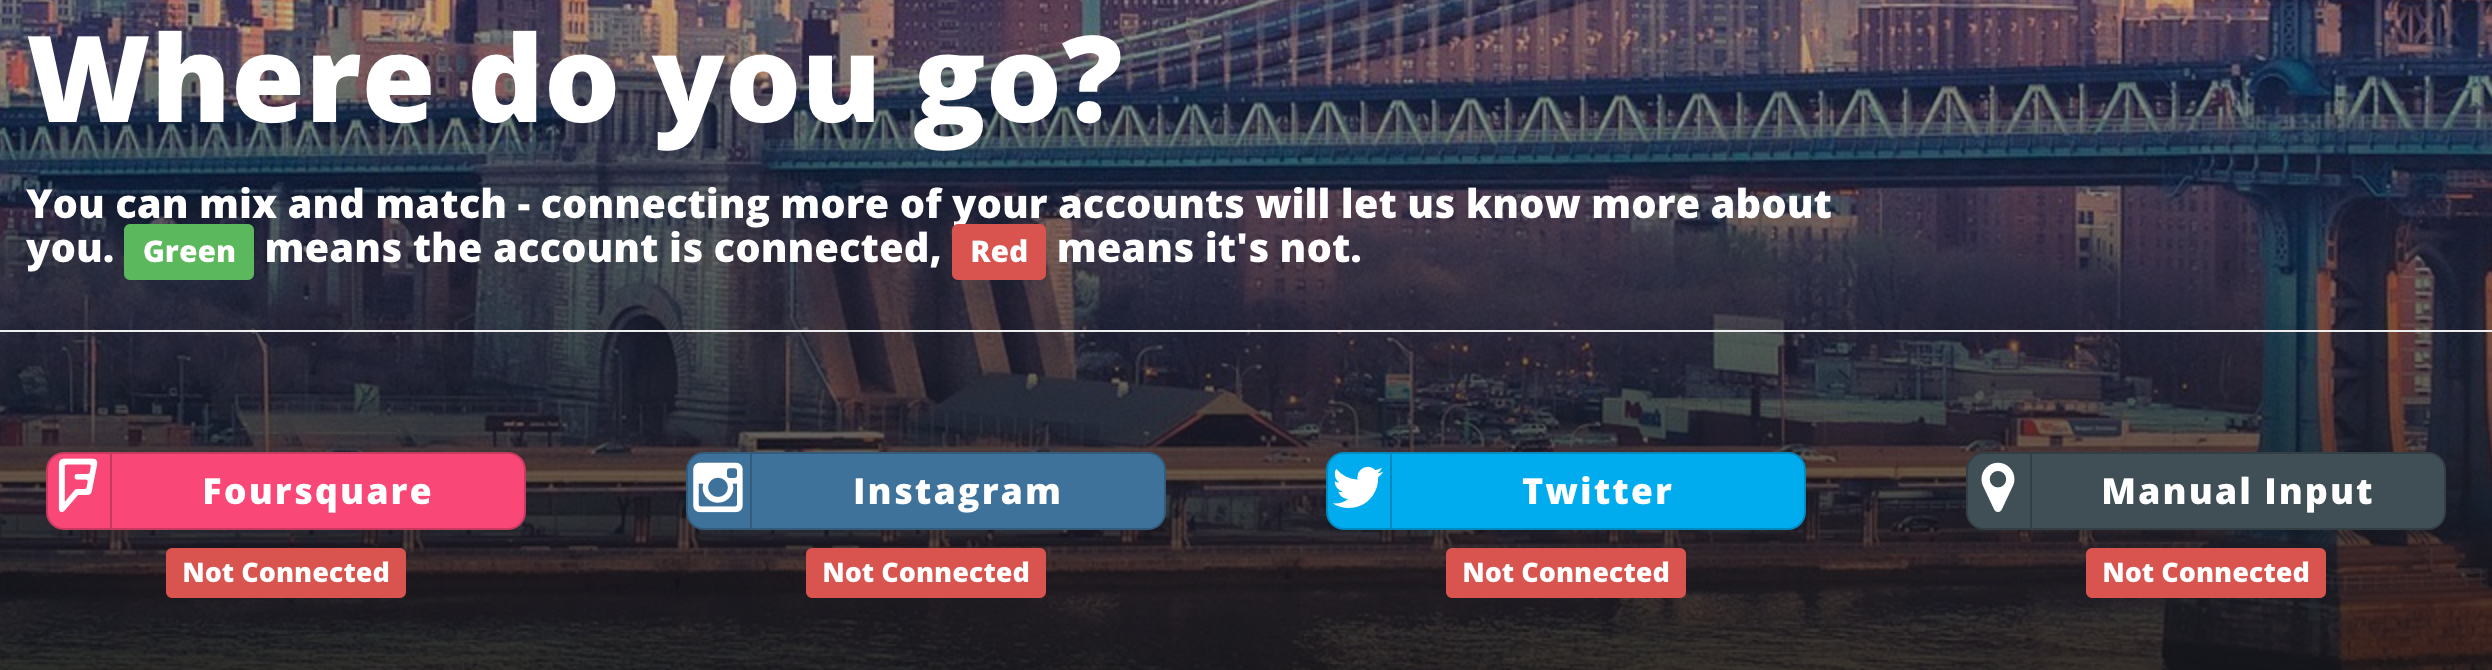
\includegraphics[width=\linewidth]{fig/findyou/connection.png}
  % \caption{The user is presented with four different ways of connecting his or her location data to the app.}
  % \label{fig:connection}

  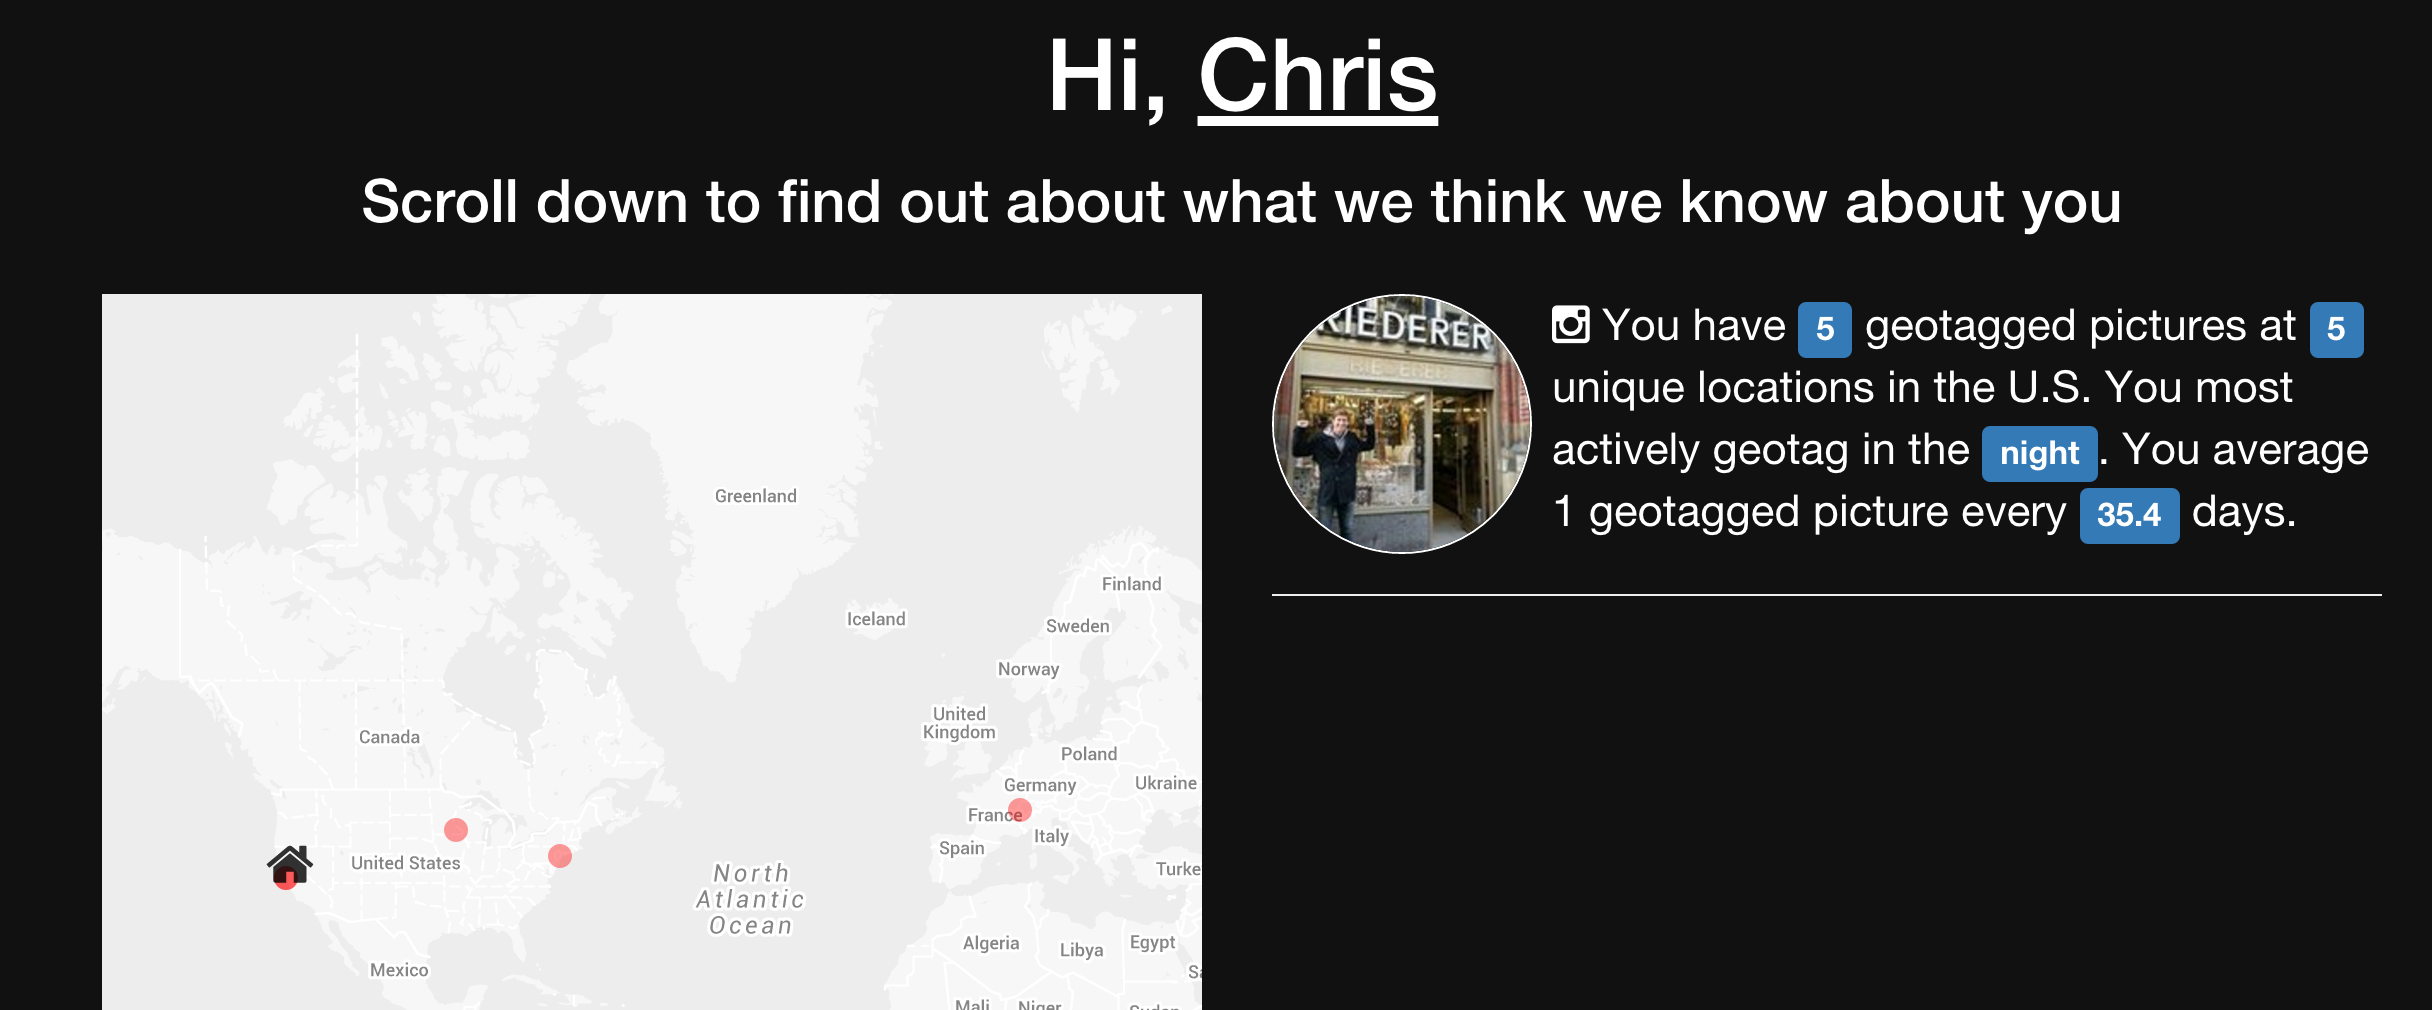
\includegraphics[width=\linewidth]{fig/findyou/overview.png}
%   % \caption{After connecting their data, the user sees an overview of their locations and imported data.}
%   % \label{fig:overview}
% % \end{figure}

  
\includegraphics[width=\linewidth]{fig/findyou/home.png}
%   % \caption{We show a specific guess for the user's home location.}
%   % \label{fig:home}

  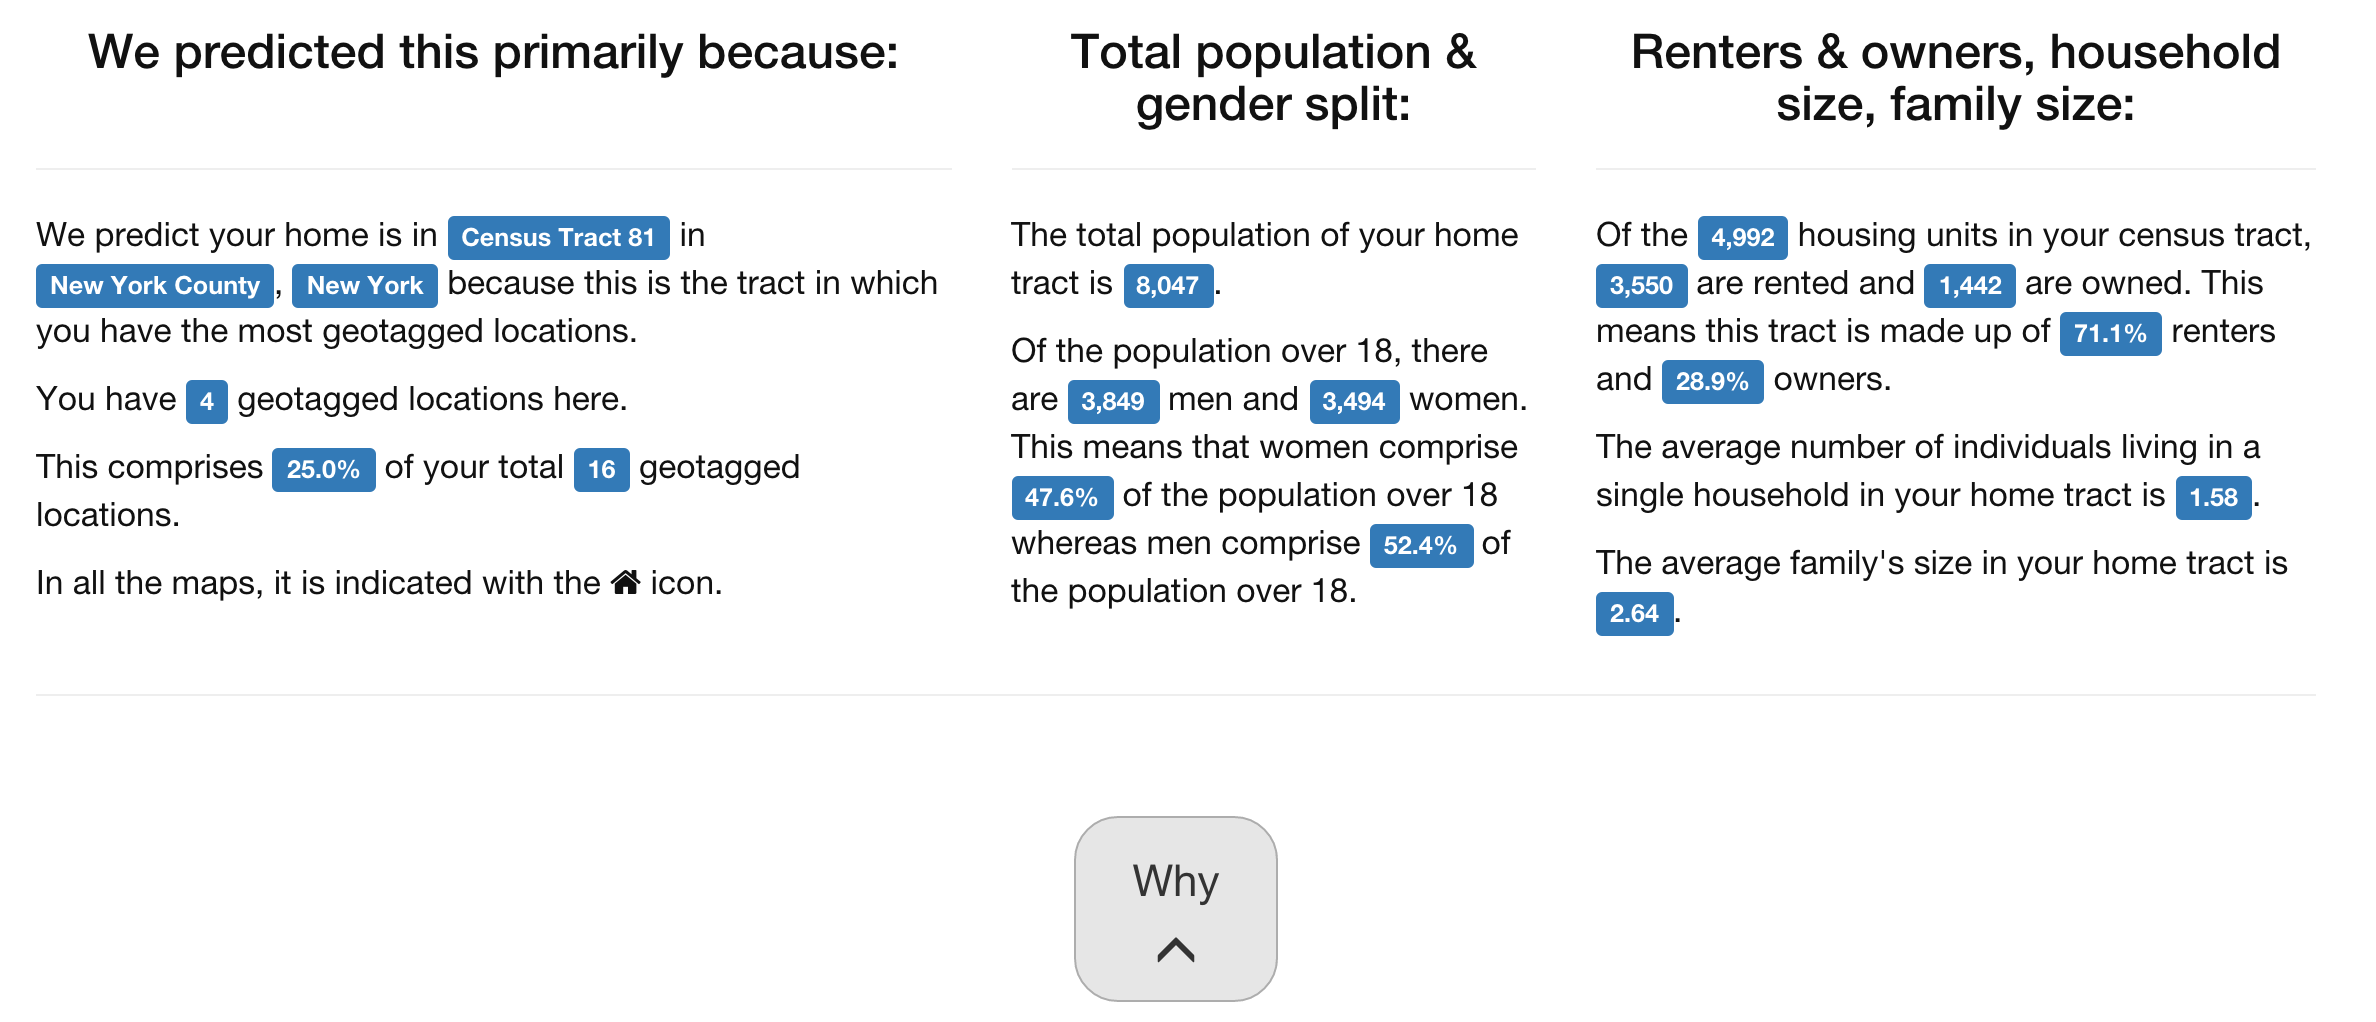
\includegraphics[width=\linewidth]{fig/findyou/home-detail.png}
%   % \caption{For all predictions, we show additional details about how we made this guess.}
%   % \label{fig:home-detail}

  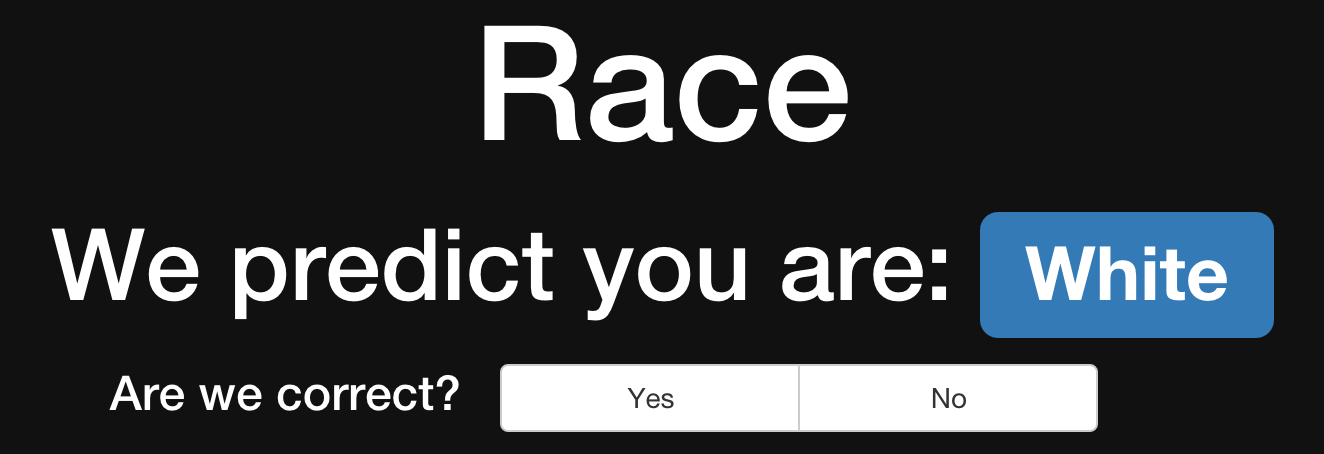
\includegraphics[width=\linewidth]{fig/findyou/race.png}
  \caption{Screenshots from the site, displaying (top to bottom) options for linking to data sources, a map showing the users' data, and predictions about home location and demographic, with prediction details.}
  \label{fig:findyou_screencap}
\end{wrapfigure}

\textbf{Site Summary} \\
When opening the site, the user is greeted with a general description of the project. After clicking through this screen, the user has the option to import their data from three different web services or to manually import data by clicking visited locations on a map. Upon importing their data, users see the distribution of their visited locations of several different demographic traits, including race, income, age group, and parental status. Finally, at the bottom of the page, users have the ability to donate their data for further research.

\textbf{Design Decisions} \\
\emph{Why did we choose these sites?}
FindYou is currently able to import data from three popular online services or manually, by a user clicking on visited points on a map. The three sites we chose are Instagram, Twitter, and Foursquare. These sites were chosen because they are all popular but also present a diversity of behaviors and different levels of focus on location. We will discuss each of these sites in turn.

\textbf{Foursquare} is a location-based social network and review site. 
Users write reviews of and give tips about locations they have visited. 
It is estimated to have 50 million users. 
Foursquare is the most ``location-centric" of our utilized web-services, as users must reveal their location to obtain any value from the service.
\textbf{Instagram} is a photo-sharing application owned by Facebook with 400 million monthly active users. 
Instagram is notable for it being primarily targeted at mobile phones; currently users cannot upload photos from a desktop or laptop computer.
The mobile focus makes it is easy for users to ``tag" photos with locations using their phone's GPS device. 
Although many users do tag their photos with location data, unlike Foursquare, it is not necessary to post a location in order to use the app.
Due to the fact that many users do tag their photos with locations, it is the second-most ``location-centric" of our three services.
\textbf{Twitter} is a microblogging service where users post 140 character texts called ``tweets". Twitter has approximately 320 million users. Through its smartphone interface, Twitter users can tag tweets with locations. Many users connect their Twitter account to other web services, such as Foursquare and Instagram, among others, which may also contain location data. The primary focus of most tweets is not about where a user currently is. Therefore, Twitter is the least location-centric. 

We additionally included an option for \textbf{manual input}. 
This option simply has users click on a map to say where they've been. 
We included this option and used this design for several reasons. 
First, we wanted users who do not use any of the three aforementioned services to be able to participate in a location information privacy audit. 
Additionally, allowing users to manually input data gives the ability for users to play with hypothetical trips or to input locations that were not tagged in the services. 
We used this design because it is easy and simple.

% In the future, we hope to connect more services and also include more advanced location-data uploading. For example, users could include data in standard geographic formats, such as GeoJSON or those used by GIS software. For the time being, we believe that our three chosen services and simple uploading methodology will provide users with an interesting and useful coverage of options.

\emph{Why did we choose to display these demographic features?}
After a user has imported at least some of their location data, we display demographic information on the places they visited. 
The features we chose to show are race, income level, age, and family make-up (number of households with children). 
The user sees a pie chart showing the average (over the user's visited locations) categorical distribution for that demographic trait. 
The site additionally displays specific details about each category for the user's most visited location. 
Technically, this works by utilizing information from the United States Census. On our server, we store information on the boundaries of each U.S. Census tract. 
We additionally have information on the make-up of each Census tract for our selected traits.
We chose these features to be interesting, surprising, and possible to infer using location data. 
Hopefully, FindYou can include additional interesting demographic features in the future. 


\begin{wrapfigure}{R}{0.49\textwidth}
  \centering
  \begin{subfigure}[b]{.48\linewidth}
    \centering
    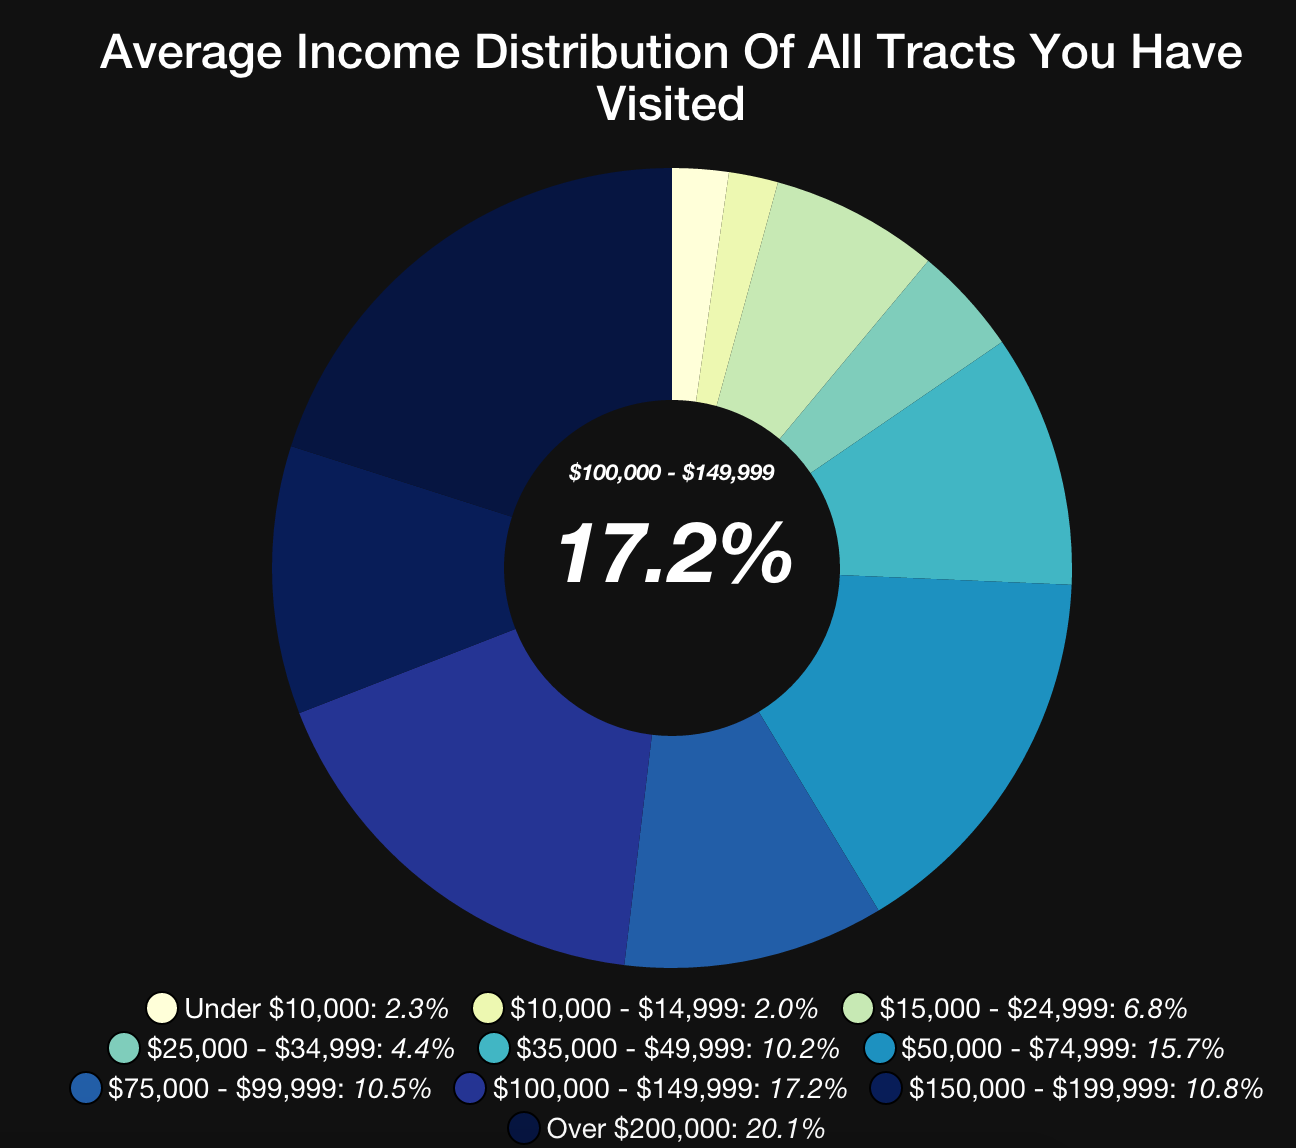
\includegraphics[width=\linewidth]{fig/findyou/donut.png}
    \caption{}
  \end{subfigure}
  \begin{subfigure}[b]{.48\linewidth}
    \centering
    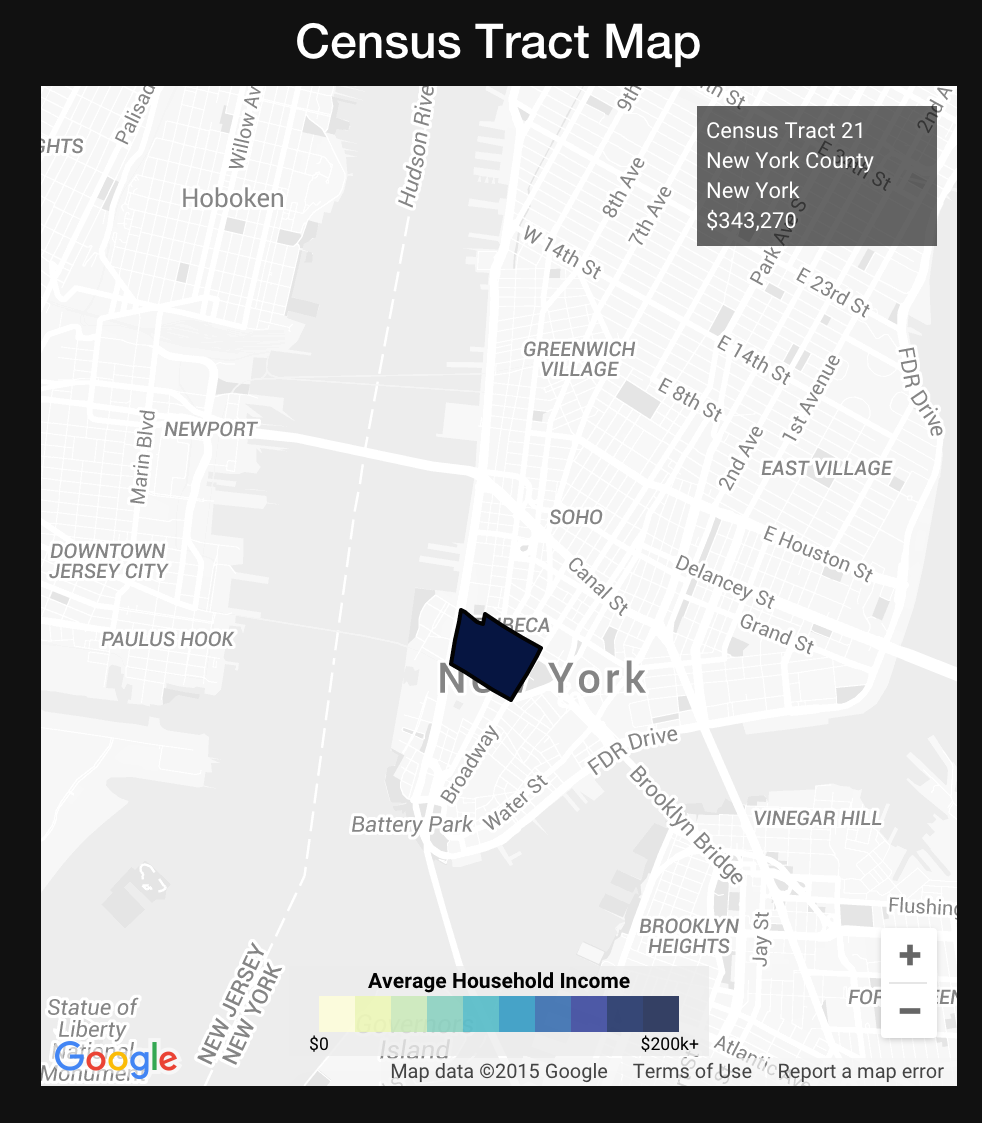
\includegraphics[width=\linewidth]{fig/findyou/tract-map.png}
    \caption{}
  \end{subfigure}
  \caption{(a) Donut graph displaying distribution of income groups visited by user, and (b) map showing tracts visited by user along with income information on each tract.}
\end{wrapfigure}

\emph{Why did we use only simple machine learning techniques?}
In addition to descriptive data about the distribution of visits in each category, we also present predictions of which category a user falls into for each demographic attribute. Although users may be interested about the demographics of the locations they visit, they might not realize that this information can be used to infer their own traits. Therefore, showing predictions is useful in and of itself, even if the predictions aren't all accurate, as it shows users that their data can be used in such inferences.
% (TODO: citation to show that users don't understand that most companies use their data?)
Driven by our goal of simplicity in explaining what's going on to the user, we use simple techniques that are intuitive for most users, as opposed to using more difficult to understand methods like SVMs or neural networks. For each demographic trait, we predict the user to be in the class to which they have the most visits. To make this concrete, consider the example of age. We break age into several categories. 
% (TODO: the categories)
We average the distribution of age categories of all the locations a user has visited, and pick the category with the largest proportion. 

\emph{How did you choose to represent locations?}
There are many different ways to represent locations, such as latitude longitudes, venues, cities, or points of interest.
Throughout the paper and the site, we use a United States Census tract as an ``atomic" location.
The United States Census partitions the country into \emph{census tracts}, which are stable geographic boundaries chosen to contain homogeneous populations.
Census tracts are typically the size of a few city blocks and might contain 4000 or fewer people.
We chose to represent all locations as a census tract for several reasons.
First, we can map any latitude longitude point into a census tract, and thus any venue with an associated lat-lon into a tract as well.
Census tracts are small enough to be targeted, but large enough to display without overwhelming the user.
Finally, they are all associated with detailed demographic information from the Census.
Throughout the site, whenever a census tract is mentioned, the user can click on it to see its geographic boundaries and demographic make-up.

%TODO(cjr): add conclusion to FindYou?

% \emph{Why only America?}
% Due to our reliance on U.S. Census data, our site currently only bases it's predictions on visits to locations in the United States. We hope to expand to other countries in the future. This presents some challenge, as each census of each country will have different types of data available, different classifications, groupings, and currencies, and different APIs. We look forward to tackling this challenge in future work. For the time being, focusing on the world's third most populous country with one standardized census and many online social network users has appeared to be a good option.

